\documentclass[12pt,a4paper]{article}
\usepackage[utf8]{inputenc}
\usepackage{amsmath}
\usepackage{amsfonts}
\usepackage{amssymb}
\usepackage{graphicx}
\usepackage{polski}
\usepackage{mathtools}
\usepackage[T1]{fontenc}
\usepackage{pdflscape}
\usepackage{graphicx}
\usepackage{caption}
\usepackage{subcaption}
\usepackage{floatrow}
\usepackage{float}
\DeclarePairedDelimiter{\ceil}{\lceil}{\rceil}

\title{Rozmieszczanie kamer bezpieczeństwa}
\author{Wiktor Franus \\ Grzegorz Staniszewski}

\begin{document}
\maketitle
\tableofcontents

\newpage
\section{Treść zadania}
Jak optymalnie rozmieścić kamery monitoringu w ustalonym pomieszczeniu (rzut z góry), aby minimalną liczbą kamer móc obserwować dowolne miejsce (z uwzględnieniem maksymalnej dopuszczalnej odległości od kamery). W rozwiązaniu należy uwzględnić możliwość zapewnienia parametryzowanej redundancji - tzn. wymagania, aby każde miejsce było obserwowane przez co najmniej $n$ kamer.

\section{Założenia}
\begin{enumerate}

\item Pomieszczenie jest wielokątem zawierającym tylko kąty o mierze 90 lub 270 stopni. Pomieszczenie reprezentowane jest przez zbiór punktów (z I ćwiartki układu współrzędnych) podanych w formie listy. Połączenie tych punktów linią, zgodnie z ich kolejnością na liście, skutkuje otrzymaniem linii łamanej ograniczającej pomieszczenie.
\item Kamery mają jednakowy zasięg reprezentowany przez kwadrat o stałej długości boku równej 2 jednostki. Współrzędne kamery są jednocześnie współrzędnymi środka tego kwadratu. Kamera musi znajdować się wewnątrz pomieszczenia i nie przenika przez ściany.
\item Wnętrze pomieszczenia zdyskretyzowane jest do zbioru punktów o współrzędnych całkowitych poprzez nałożenie siatki o gęstości 1 jednostki.
\end{enumerate}

\section{Przestrzeń przeszukiwań}
\begin{itemize}
	\item Elementem przestrzeni przeszukiwań jest zbiór kamer wraz z ich położeniem.
	\item Przejście do sąsiedniego elementu możliwe jest poprzez:
	\begin{itemize}
		\item zmianę współrzędnych x lub y jednej z kamer o 1 jednostkę
		\item dodanie nowej kamery w losowym miejscu
		\item usunięcie jednej kamery
	\end{itemize}
\end{itemize}


\newpage
\section{Funkcja celu}
Informacje znane dla danej instancji problemu: \\
$n_{kmin}$ - minimalna teoretyczna liczba kamer wymagana do pokrycia danego pomieszczenia \\
$X$ - zbiór punktów reprezentujących wnętrze pomieszczenia \\
%
\newline
Parametry do strojenia: \\
$\alpha$ - zysk z pokrycia $\frac{1}{100}$ pola powierzchni pomieszczenia \\
$\beta$ - koszt użycia nadmiarowej kamery \\
$r_{min}$ - minimalna liczba kamer pokrywająca każde miejsce w pomieszczeniu \\
%
\newline
Zadanie polega na maksymalizacji funkcji: \\
$$f(p, k, r) = \alpha * p - \beta * k - \frac{1}{r_{min}} * r $$ 
gdzie: \\
$p$ - stosunek powierzchni pokrytej przez kamery do powierzchni pomieszczenia \\
$k$ - stosunek nadwyżki liczby kamer do $n_{kmin}$, obliczany wg. wzoru: \\
\indent $k = \frac{max(0, n_k - n_{kmin})}{n_{kmin}}$, gdzie $n_k$ - liczba kamer w aktualnym stanie \\\\
$r$ - średni stopień niespełnienia warunku redundancji dla punktu z wnętrza pomieszczenia, obliczany wg. wzoru: \\
\indent $r = \frac{\sum_{x \in X}^{} max(0, r_{min} - r_x)}{|X|}$, gdzie $r_x$ - liczba kamer pokrywających punkt $x$

%
\section{Przykład}
\begin{center}
	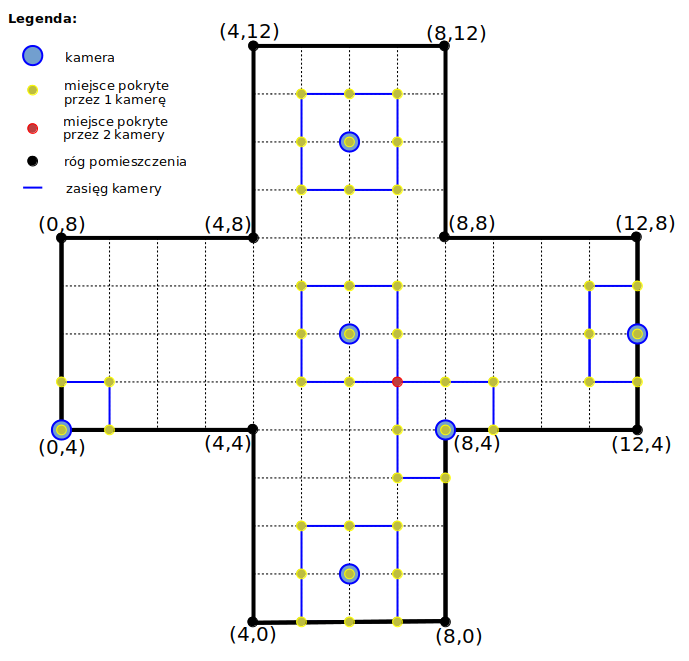
\includegraphics[scale=0.6]{img/example.png}
\end{center}


\begin{itemize}
	\item Wartości parametrów:\\
	$\alpha = 1$\\
	$\beta = 1$\\
	$r_{min} = 1$
	\item Informacje obliczone dla powyższego pomieszczenia:\\
	pole powierzchni pomieszczenia: 80\\
	$n_{kmin} = \frac{80}{2*2} = 20$\\
	$|X| = 105$
	\item Obliczenie wartości funkcji celu dla stanu z rysunku:\\
	Liczba kamer użytych: 6\\
	Pole powierzchni pokryte przez kamery: 18\\
	$p = \frac{18}{80} = 0.225$\\
	$k = \frac{max(0, 6-20)}{20} = \frac{0}{20} = 0$\\
	$r = \frac{44*0 + 61*1}{105} = \frac{61}{105} = 0.58$\\
	$f(p, k, r) = 1*0.225 - 1*0 - 1*0.58 = -0.355$
\end{itemize}

\section{Metaheurystyka}
Element początkowy przestrzeni przeszukiwań jest zbiorem zawierającym $n_{kmin}$ (obliczane jako stosunek pola powierzchni pomieszczenia do pola powierzchni zasięgu jednej kamery, zaokrąglany do jedności w górę) kamer rozmieszczonych losowo wewnątrz pomieszczenia.\\
Do rozwiązania problemu użyjemy algorytmu symulowanego wyżarzania. Przy odpowiednio dobranych parametrach metoda ta, w porównaniu do algorytmów wspinaczkowych, daje większą szansę na znalezienie optymalnego rozwiązania, ponieważ zmniejsza ryzyko zatrzymania się w ekstremach lokalnych. W początkowej fazie przeszukiwania przestrzeni dopuszczalne jest przechodzenie do stanów gorszych (o mniejszej wartości funkcji celu). Wraz z rosnącą liczbą iteracji obszar poszukiwań jest ograniczany, a algorytm bardziej skupia się na poprawie bieżącego rozwiązania.

\section{Przewidywane wyniki pracy}
Przeprowadzona zostanie seria eksperymentów z różnymi wartościami parametrów $\alpha$, $\beta$, $r_{min}$ na kilku instancjach problemu (różne pomieszczenia). Sporządzone zostaną wykresy przedstawiające wartość funkcji celu oraz liczbę użytych kamer w zależności od liczby wykonanych iteracji. Sprawdzony zostanie wpływ parametru temperatury poprzez zmianę jego wartości początkowej oraz funkcji wygaszania.

\end{document}